In this section we present the results from our simulations experimenting performance impa



-	Performance gain (IPC) \\
-	LFMR, MPKI \\
-	Comparison to other Special Kernels (Lulesh)





\begin{figure}[!th]
 \centering
  %\vspace*{-2.em}

   \subfloat[IPC.\label{subfig-2:cades}]{
    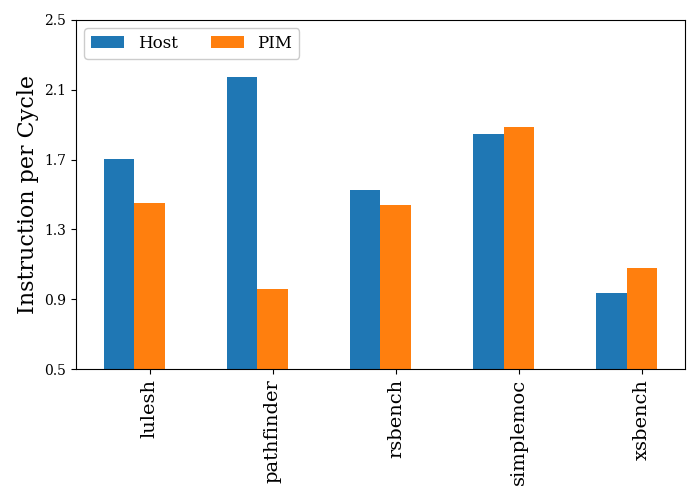
\includegraphics[width=1\linewidth,scale=1.0,keepaspectratio]{MEMSYS22/figures/ipc.png}
  }
  
  \subfloat[MPKI.\label{subfig-2:dgx}]{
    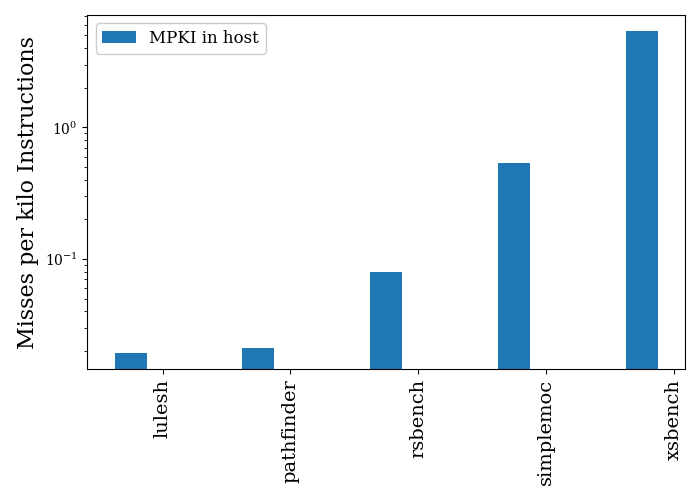
\includegraphics[width=1\linewidth,scale=1.0,keepaspectratio]{MEMSYS22/figures/mpki.png}
  }
  
   \subfloat[LFMR.\label{subfig-2:crusher}]{
    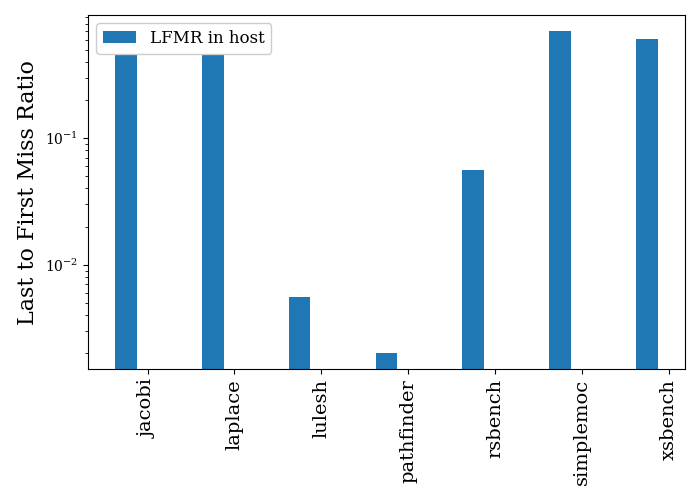
\includegraphics[width=1\linewidth,scale=1.0,keepaspectratio]{MEMSYS22/figures/lfmr.png}
  }
  
   \vspace{-.05in}
   \caption{Impact of PIM in different applications. Visible correlation between performance improvement using PIM and MPKI and LFMR.
   }
 \vspace{-.1in}
 \label{fig:expr:pim}
 \vspace{-1em}
\end{figure}



%
%\begin{figure}[t!]
%\hspace*{-9.5cm}
%\centering
%\includegraphics[width=\textwidth, height=60mm]{figure/Set1.pdf}
%%\caption{ST-1.2 Configuration (floating point benchmarks): Speedup ranges from 0\% (tonto) to 7.4\% (milc), and it is 2.7\% on average.}
%\label{fig:Set1}
%\end{figure}
%
%
%\begin{figure}[htbp]
%  
%\centering
%\includegraphics[width=\textwidth, height=60mm]{figure/Set2.pdf}
%%\caption{ST-1.2 Configuration (floating point benchmarks): Speedup ranges from 0\% (tonto) to 7.4\% (milc), and it is 2.7\% on average.}
%\label{fig:Set2}
%\end{figure}
%
%
%\begin{figure*}[t!]
%\centering
%\includegraphics[width=\textwidth, height=60mm]{figure/Set3.pdf}
%%\caption{ST-1.2 Configuration (floating point benchmarks): Speedup ranges from 0\% (tonto) to 7.4\% (milc), and it is 2.7\% on average.}
%\label{fig:Set3}
%\end{figure*}
%
%%\vspace{5cm}
%\newpage
%
%\begin{figure}[H]
%\centering
%\includegraphics[width=\textwidth, height=60mm]{figure/Set4.pdf}
%%\caption{ST-1.2 Configuration (floating point benchmarks): Speedup ranges from 0\% (tonto) to 7.4\% (milc), and it is 2.7\% on average.}
%\label{fig:Set4}
%\end{figure}








